\documentclass[10pt,twocolumn,letterpaper]{article}

\usepackage{iccv}
\usepackage{times}
\usepackage{epsfig}
\usepackage{graphicx}
\usepackage{amsmath}
\usepackage{amssymb}

% Include other packages here, before hyperref.

% If you comment hyperref and then uncomment it, you should delete
% egpaper.aux before re-running latex.  (Or just hit 'q' on the first latex
% run, let it finish, and you should be clear).
\usepackage[pagebackref=true,breaklinks=true,letterpaper=true,colorlinks,bookmarks=false]{hyperref}

% \iccvfinalcopy % *** Uncomment this line for the final submission

\def\iccvPaperID{****} % *** Enter the ICCV Paper ID here
\def\httilde{\mbox{\tt\raisebox{-.5ex}{\symbol{126}}}}

% Pages are numbered in submission mode, and unnumbered in camera-ready
\ificcvfinal\pagestyle{empty}\fi
\begin{document}

%%%%%%%%% TITLE
\title{High-Accurate Segmentation of Shape Constrained Object}

\author{First Author\\
Institution1\\
Institution1 address\\
{\tt\small firstauthor@i1.org}
% For a paper whose authors are all at the same institution,
% omit the following lines up until the closing ``}''.
% Additional authors and addresses can be added with ``\and'',
% just like the second author.
% To save space, use either the email address or home page, not both
\and
Second Author\\
Institution2\\
First line of institution2 address\\
{\tt\small secondauthor@i2.org}
}

\maketitle
%\thispagestyle{empty}


%%%%%%%%% ABSTRACT
\begin{abstract}
   Object segmentation has recently made great progress due to powerful features extracted using deep convolutional neural networks (CNNs).
   However in many practical scenarios, prior shape constraint about segmented object is usually available.
   Incorporating such prior knowledge into CNNs architecture to obtain the accurate morphological shape is desirable, such as vesicle segmentation.
   In this paper, we propose an effective shape constrained network (scnet) to constrain all the components of a segmentation to satisfy the prior knowledge.
   Specifically, a divide-and-conquer strategy is adopted by breaking down the segmentation into object orientation and outline depiction subtask, which is analogy to RPN in object detection.
   Furthermore a joint max pooling operation is developed to fuse the orientation and outline results into a compact form, which can be directly transformed to the segmentation result.
   The whole process is trained end-to-end and residual error can be correctly propagated.
   Our proposed method is generic as it is further used for object detection task by treating detection bounding box as rectangular object to be segmented.
   Experimental results will prove the effectivity and general of our method.
   Code is made publicly available at \url{http://www.pamitc.org/documents/mermin.pdf}..

\end{abstract}

%%%%%%%%% BODY TEXT
\section{Introduction}
Image segmentation is a challenging task which aims at segmenting the objects from complex background.
In practical application, it often occurs that there are many prior constraints on object shape, such as elliptical cell, polygonal bricks and rectangular tiles.
Especially for biological image, most membrane structure in one Electron microscopy (SEM) images have a similar shape.
For example, a typical presynaptic structure contains dense vesicles of different type, which is crucial for estimating the synaptic activity \cite{Fernandez-Busnadiego2010}\cite{Fernandez-Busnadiego2013}.
Accurate segmentation of these vesicles is a crucial pre-requisite step to obtain reliable morphological statistics, including vesicle position, inclination angle, length of major axis.

Nevertheless, this task is quit challenging for several reasons.
First, the objects such as vesicle or bricks usually get dense together, which make it easily suffer from serious touching problem \cite{Chen2016}, as shown in Fig.
Second, since the shape of objects is usually concise and compact, demand on boundary region segmentation is much higher, which is more difficult for learning.
Third, exact morphological statistics of objects are desired to be directly obtained from the network, instead of additional manual measuring in conventional strategy.

Most existing segmentation methods using deep convolutional neural networks (CNNs) \cite{Chen2014},\cite{Zhao2016},\cite{Arnab2016},\cite{Chen2016},\cite{Zheng} to predict a label for each pixel in an image.
However they do not model the interactions between output variables directly, thus the boundaries of segmentation object are usually coarse and smooth, which is terrible for some object with sharp outline shape.
Moreover without any shape constraint on segmenting objects, contiguous objects are easily touching each other, as shown in Fig.
\cite{Chen2016a} solves this problem by using edge prediction to cleave the touching cells, while \cite{Ronneberger2015} add the loss weights around the boundary regions.
However the boundaries obtained by cleaving is coarse and exact morphological statistics still needs further operation.
Some methods for segmenting specific shape structure are not deep neural architecture, which commonly segment multiple structures sequentially and can't be globally optimized among the whole input image. \cite{Gulshan2010},\cite{Sirinukunwattana2015},\cite{Royer2016},\cite{Veksler2008},\cite{Strekalovskiy2011},\cite{Gorelick2014}.
Few study has successfully incorporating these shape constraint into the deep convolutional neural networks (CNNs) as an unified framework.
\begin{figure*}\label{Fig2}
\begin{center}
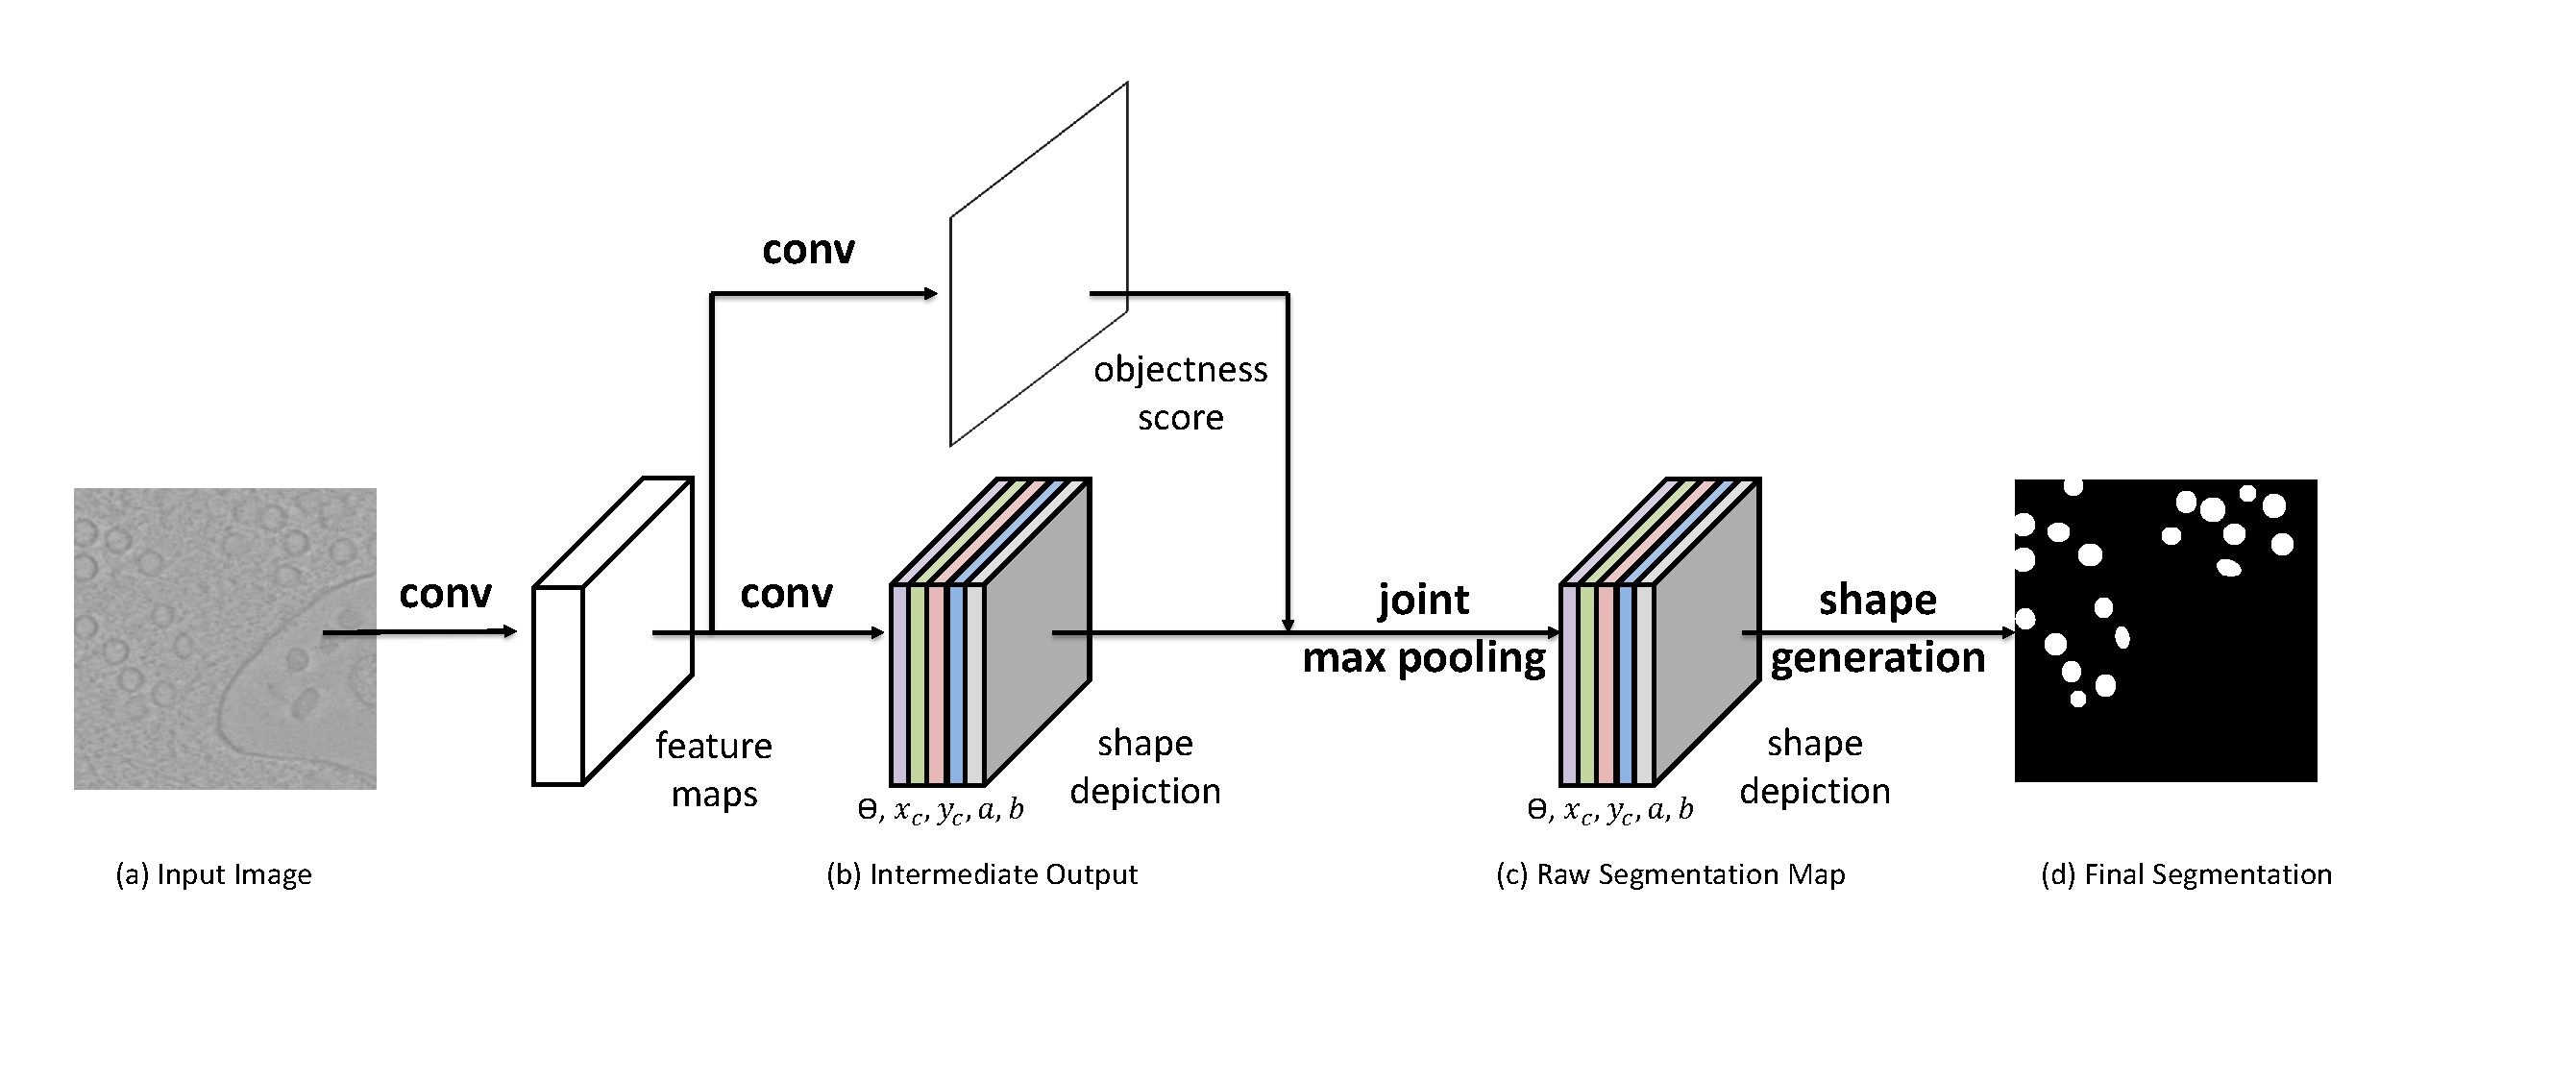
\includegraphics[width=6.8in]{Fig2.pdf}
\end{center}
   \caption{Overview of our proposed scnet. Given an input image (a), shape constraint net first use deeplab to get the feature map and generate two intermediate outputs (b) including objectness score and shape depiction. Then the joint max pooling operation is applied to fuse (b) into a raw segmentation map, which is finally transformed to final segmentation (d) by shape generation layer. The whole network can be jointly trained end-ro-end.}
\end{figure*}
%Despite important of these prior shape knowledge, few work focus on introducing them into the deep convolutional neural networks (CNNs), which can be jointly trained end-to-end.

In this work, we propose the first shape constraint network (scnet) to segment dense objects with certain shape constraint, while simultaneously resulting in corresponding morphological statistics for each object.
We formulate the shape constraint as a set of parameters, which can depict the outline shape of object.
Analogy to Region Proposal Network in \cite{Ren2015}, the previous part of our scnet produce a set of parameterized shape depiction, each with an objectness score
The insight is to divide this challenging task into two easier part, one designed for finding out all the possible objectness region, another one designed for depicting the ourline shape of possible object.
In order to make our scnet effectively using these two abilities, a joint max pooling operation was developed to fuse above two outputs into an unified form results.
The function of joint max pooling method is to impose a consistency of distribution between objectness score and shape depiction, while reduce training difficulty by only focusing attention on part of the image.
Finally parameterized shape description will be transformed into a general segmentation results by our shape generation layer.
The whole network can be jointly trained end-to-end, and intermediate results (parameterized shape depiction) can be directly extracted as morphological statistics of object shape.
Furthermore, our scnet can be easily converted to solve the object detection task, such as scene text detection, by regarding the detection bound box as a rectangular object.

   %Object detection has recently witnessed great progress due to powerful region-based detectors with deep convolutional neural networks(CNNs).
   %However existing region-based detectors such as Faster R-CNN lack intrinsic consistency between rectangular proposals and their objectness scores.
   %This makes the rectangular proposals from RPN corresponding to the highest scores not the most accurate, which should be further modified by Fast R-CNN.

%parameterized shape depiction and objectness scores can be directly leant from the final segmentation results, without needing preparing any other data.

%   The accurate segmentation is of great importance in some segmentation tasks with strict shape constraints.
%   Precise shape parameters of synaptic vesicle has recently been used by neurologist to study the synaptic activity.
%   Hight accurate segmentation of vesicles from Electron microscopy (SEM) images is a crucial step to distinguish subtle variations among different vesicles.
%-------------------------------------------------------------------------

\section{Joint Region Proposal Netwrok}
\subsection{Overview}
The complete pipeline of proposed method is illustrated in Figure \ref{Fig2}.
They are jointly trained end-to-end and consists of three components.

Analogy to famous Region Proposal Network \cite{Ren2015}, the first component takes an image as input and produces a coarse objectness score map and associated shape parameters map.
Different to original RPN, the rectangular proposals are replaced by outline shape parameters of the object that it belongs to, and a dense prediction strategy is adopted which predicts an object for each position of input image.
The objectness score is the predicted probability of the position being inside an object and shape depiction is a set of parameters, which depict outline shape of possible object it belonging to.
Our model first find out all the possible object from predicted score map, and then depict its predicted shape by the shape parameter map.
For instance in vesicle segmentation, the object shape depiction can be formulated by $[\theta,x_c,y_c,a,b]$, including the angle of major axis, coordinate of center point and two elliptical axis length of the object as in Figure \ref{Fig2}, which restricts the segmented object to be ellipse.
Especially, if only the shape constraint can be formulated by parameterization, our scnet can integrate this constraint into the network.
The architecture of the first component is based on the publicly available DeepLab-LargeFov model \cite{Chen2014}, which modifies VGG-16 net \cite{Simonyan2014} to be FCN \cite{Long2015} and introduces zeros into the filters to enlarge its Field-Of-View.
At the end of DeepLab, another regression layer is introduced to predict shape parameter.

We develop a joint max pooling operation as our second component, which fuses the results from first components into a raw segmentation map.
Especially, the existing region-based detectors lack intrinsic consistency, of which the results were dividedly optimized.
% between rectangular proposals and their objectness scores.
%From the loss function defined in [], it can be discovered that their results were dividedly optimized.
However our joint max pooling can impose a consistency on the preceding outputs, restricting the highest score corresponding to the most accurate proposal.
Furthermore, the implementation of joint max pooling is very efficient, since the residual error is sparse and can be correctly propagated.
The whole joint max pooling operation can be easily expanded to other pooling operations.

%In other words, the region proposals are rectangular proposals that RPN think the most likely correct.
%However from the loss function defined in [], we find that the association between proposal and corresponding score is too weak.
%\begin{eqnarray}\label{rpnloss}
%\begin{aligned}
%L(\mathbf{x})=& \frac{1}{N_{cls}}\sum_{i,j}\sum_k L_{cls}(p_{i,j,k},p^*_{i,j,k})+\\
%&\lambda\frac{1}{N_{reg}}\sum_{i,j}\sum_k p_{i,j,k}^*L_{reg}(t_{i,j,k},t^*_{i,j,k})\\
%\end{aligned}
%\end{eqnarray}
%where $i$, $j$ are pixel coordinates and $k$ is the index of an anchor,
%$p_{i,j,k}$ is the predicted probability of anchor $k$ at position $x_{i,j}$ being an object.
%The ground-truth label $p_{i,j,k}^*$ is $1$ or $0$ if the anchor $k$ is positive or negative.
%$t_{i,j,k}$ is a vector representing the parameterized coordinates of predicted bounding box.
%the loss function of RPN equally penalizes all the rectangular proposals whose $p_{i,j,k}^*=1$

The third component in our framework is a novel object generation layer, which transforms the raw segmentation map to the final segmentation prediction.
The shape parameters map can be learnt directly from the segmentation results without preparing any other ground truth.
Therefore, the accurate statistical shape parameters of each object can be very conveniently obtained.

%The first component in [] is the Region Proposal Network (RPN), which takes an image as input and outputs a set of coarse rectangular object proposals with an objectness score.
%Different from original RPN in [], we add a joint pooling operation at the tail of network, as illustrated in Fig.
%Although implementation of joint pooling is very efficiently, it can effectively impose the consistency and sparsity on the outputs of RPN.
%Especially in this paper, joint pooling refers to joint max-pooling, but it can be easily expanded to other pooling operation.

We first introduce our joint pooling operation in Sec. 3.2, and then we extend it to a trainable system in Sec. 3.4.
Finally the object generation is applied to generate the final object segmentation result.

%\subsection{Region Proposal Network}
%For object detection task, the target of RPN is to provide as correct region proposals as possible to subsequent region classifier.
%In other words, the region proposals are rectangular proposals that RPN think the most likely correct.
%However from the loss function defined in [], we find that the association between proposal and corresponding score is too weak.
%\begin{eqnarray}\label{rpnloss}
%\begin{aligned}
%L(\mathbf{x})=& \frac{1}{N_{cls}}\sum_{i,j}\sum_k L_{cls}(p_{i,j,k},p^*_{i,j,k})+\\
%&\lambda\frac{1}{N_{reg}}\sum_{i,j}\sum_k p_{i,j,k}^*L_{reg}(t_{i,j,k},t^*_{i,j,k})\\
%\end{aligned}
%\end{eqnarray}
%where $i$, $j$ are pixel coordinates and $k$ is the index of an anchor,
%$p_{i,j,k}$ is the predicted probability of anchor $k$ at position $x_{i,j}$ being an object.
%The ground-truth label $p_{i,j,k}^*$ is $1$ or $0$ if the anchor $k$ is positive or negative.
%$t_{i,j,k}$ is a vector representing the parameterized coordinates of predicted bounding box.
%
%On the one hand, the loss function of RPN equally penalizes all the rectangular proposals whose $p_{i,j,k}^*=1$.
%In fact if only one of rectangular proposals, corresponding to the same bounding box, is correct and output, the result is just correct.
%On the other hand, the residuals of the rectangular proposal of top objectness score, which will be propagated to fast R-CNN, maybe not the smallest.
\subsection{Joint max pooling}
\begin{figure}[t]
\begin{center}
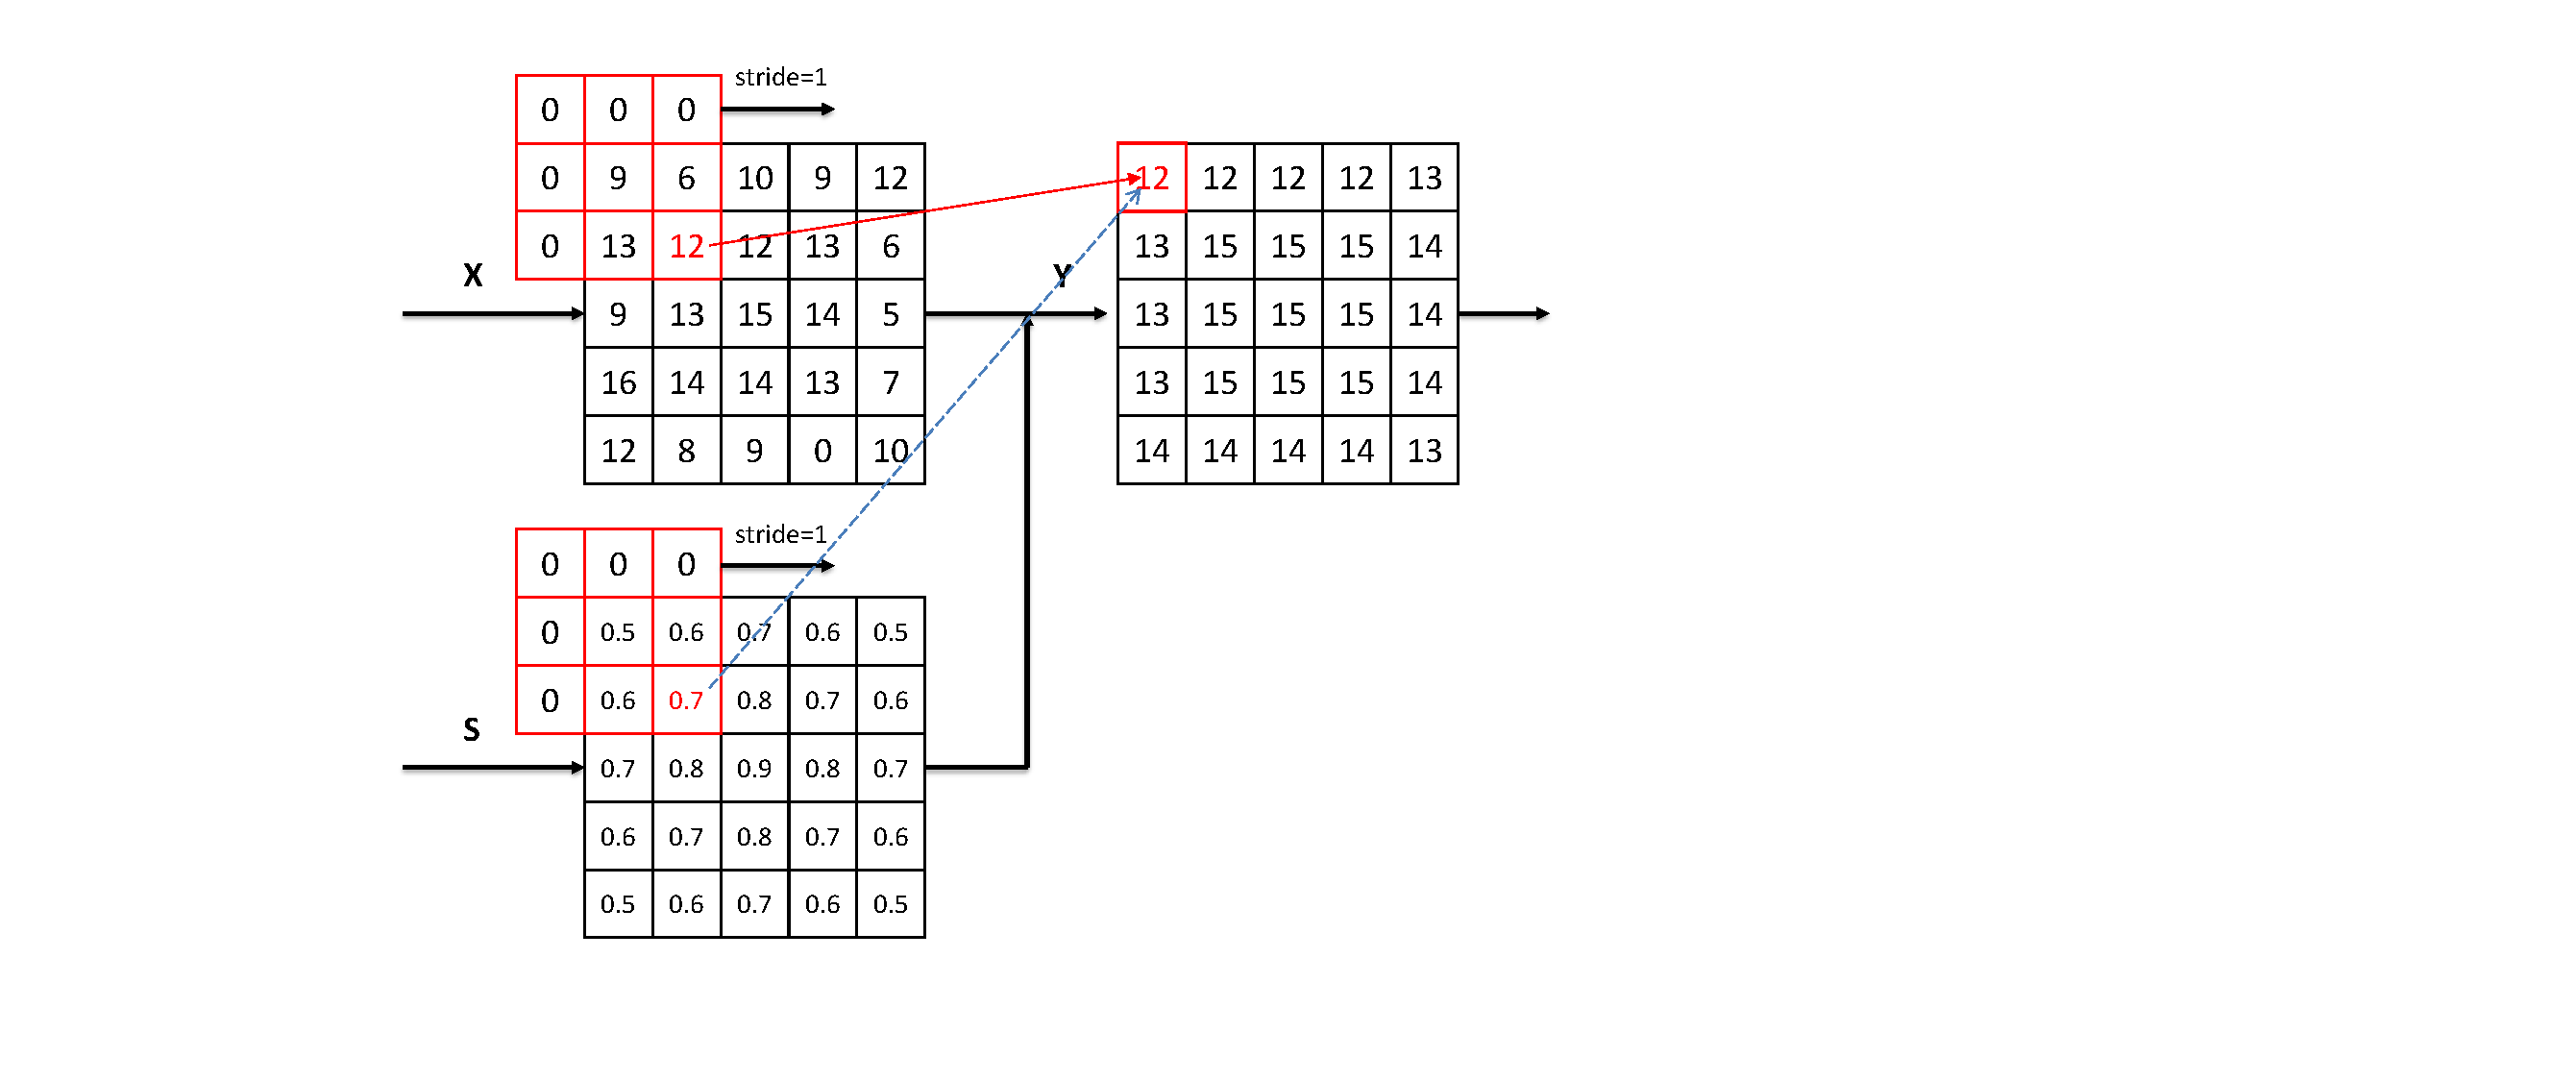
\includegraphics[width=3.4in]{Fig3.pdf}
   %\includegraphics[width=0.8\linewidth]{egfigure.eps}
\end{center}
   \caption{A diagram of joint max pooling process in Eq .\ref{sjmp}.
   Inputting two matrices $\mathbf{X}$ and $\mathbf{S}$, a $3\times3$ max pooling window is applied to $\mathbf{S}$ with padding operation for the top left position.
   Recording the position of the max valve $0.7$ in $\mathbf{S}$, we output the value $12$ in corresponding position in $\mathbf{X}$.
   The process is repeated with pooling window sliding.}
\label{F3}
\end{figure}
Original max pooling operation takes a $2$-$D$ signal $\mathbf{X}$ as input and outputs a filtered signal $\mathbf{Y}$:
\begin{eqnarray}\label{mp}
\begin{aligned}
y_{\mu,\nu} = max(\{x_{i,j}|x_{i,j}\in \mathbf{P}\})
\end{aligned}
\end{eqnarray}
where $\mathbf{P}$ is a local field of $\mathbf{X}$ associated to $y_{\mu,\nu}$ in $\mathbf{Y}$:
Intuitively, information carried by the strongest $x$ in $\mathbf{X}$ can be propagated to next layer, while the other $x$ are abandoned.
And the max pooling process can be further expressed as:
\begin{eqnarray}\label{jmp}
\begin{aligned}
y_{\mu,\nu} = \sum_{i,j}x_{i,j}b_{i,j}~~~~~~~x_{i,j}\in \mathbf{P},b_{i,j}\in \mathbf{B}
\end{aligned}
\end{eqnarray}
where $\mathbf{B}$ is a binary matrix, whose elements are all zero except for the position where $x$ is maximum in $\mathbf{P}$.
In this formulation, $\mathbf{B}$ acts like an "indictor" determining which $x$ can be propagated to next layer.
And in Eq \ref{jmp}, the criterion of indictor is who is bigger.
Especially most existing pooling methods can be interpreted by an "indictor" with different judgment criteria.
Based on this intuition, a natural question arises that whether the criterion can be learnt in terms of different task.
That is, the indictor is no longer fixed before task beginning and can be learnt during training stage, in which way, the pooling operation will be more powerful and flexible.

Followed by this discussion, the joint max pooling method is proposed, as illustrated in Figure \ref{F3}.
The passing $x$ is no longer determined by its value, instead we learn a more intelligent "indictor" to determine which $x$ is more valuable.
The whole process can be regarded as a split version of pooling, whose input is split into two parts.
In practice, $\mathbf{B}$ is hard to be directly learnt as binary, instead we learn a score matrix $\mathbf{S}$ that evaluates the importance of information carried by $x$.
Therefore only the information with highest importance can be propagated:
\begin{eqnarray}\label{max}
\begin{aligned}
\overline{s} = max(\{s_{i,j}|s_{i,j}\in \mathbf{S}\}\\
\end{aligned}
\end{eqnarray}
\begin{eqnarray}\label{sjmp}
\begin{aligned}
y_{\mu,\nu} = \sum_{i,j}x_{i,j}g(s_{i,j}-\overline{s})~~~~x_{i,j}\in \mathbf{P}
\end{aligned}
\end{eqnarray}

\begin{eqnarray}\label{sign}
\begin{aligned}
g(t)&=&\left\{\begin{array}{cc}
1&if~t>=0\\
0&else\\
\end{array}\right.
\end{aligned}
\end{eqnarray}

The intrinsic consistency of join max pooling, imposing on its two inputs, is very suitable to associate shape depiction and object location together, as only the shape predictions with highest score can be propagated and updated.
As shown in Fig, $\mathbf{X}$ refers to the predicted shape parameters map, while $\mathbf{S}$ is the objectness score map.
Each channel of shape parameters map $\mathbf{X}$ shares the $\mathbf{S}$.
Explicitly, we use kernel size $7\times 7$ with stride $1$ and iterate several times to let the shape prediction with high score cover a broader area.
And the output of joint pooling is a new shape prediction map, of which those predictions with low score have been all filtered out.

Moreover in a natural image, most of the area is background containing no object, and predicting shape in these regions is a wasting of energy.
Eq. \ref{jmp} still output those predictions with local max score, although they are such low scores that we believe it's background.
Therefore Eq. \ref{sjmp} is further improved by:
\begin{eqnarray}\label{fjmp}
\begin{aligned}
y_{\mu,\nu}&=&\left\{\begin{array}{cc}
\sum_{i,j}x_{i,j}g(s_{i,j}-\overline{s})& if~\overline{s}\geq\tau\\
0& else
\end{array}\right.
\end{aligned}
\end{eqnarray}

where $\tau$ is the min threshold of score that is believed to be inside the objective region.
If $\overline{s}$ is lower than threshold $\tau$, all the $y_{\mu,\nu}$ associated to $\mathbf{P}$ will be set to $0$, which means that all the $x_{i,j}\in\mathbf{P}$ belongs to background.

Our joint max pooling operation is effective.
On the one hand, the joint pooling method reduces the difficulty of learning shape predictions, since only the positions with highest objectness score are required to predict accurate shape parameters.
Besides, the information of the region with high objectness score is more abundant.
On the other hand, as all the residual errors have been converged into the positions with high score, the shape prediction in these positions will be more accurate, which will be illustrated in 3.3.

\subsection{Trainable joint pooling operation}
One important contribution of our joint pooling is that the residual error can be correctly back propagated to its two inputs.
This makes the joint pooling operation be a trainable layer in any network architecture and our scnet become a fully trainable system.

The forward pass of Eq. \ref{fjmp} is illustrated in Figure \ref{F3} and next we will demonstrate the back propagation of joint max pooling backpropagation in a general form.
Exactly, the objective of back propagation should be:
(i) improving the objetness scores of the object area;
(ii) minimizing the error of predicting shape parameters of positions with local highest objectness score.
(iii) making the local maximum points in objectness score map be sparse and moving them to the center of object as far as possible.

The third objective is to further reduce the calculation and difficulty of learning for shape predicting.
Specially in Fig, each objectness score map is assumed to not only influence the output but also feeds a subsequent layers, thus also receiving gradient contributions $\frac{\partial L}{\partial s_{i,j}}$ from the next layer during back-propagation.
Defining $\mathbf{U}$ as the $\{y_{\mu.\nu}\}$ set related to $x_{i,j}$ and $m$ as the size of $\mathbf{U}$, the back propagation can be expressed by:
\begin{eqnarray}\label{bpx}
\begin{aligned}
\frac{\partial L}{\partial x_{i,j}}=\left\{\begin{array}{cc}
\frac{1}{m}\sum\limits_{y_{\mu,\nu}\in\mathbf{U}}\frac{\partial L}{\partial y_{\mu,\nu}} & if~s_{i,j}\geq max(\overline{s},\tau) \\
0& else\\
\end{array}\right.
\end{aligned}
\end{eqnarray}
if $s_{i,j}\geq max(\overline{s},\tau)$:
\begin{eqnarray}\label{bps1}
\begin{aligned}
\frac{\partial L}{\partial s_{i,j}}&=\frac{\partial L}{\partial s_{i,j}}+\frac{1}{m}\sum_{y_{\mu,\nu}\in\mathbf{U}}\frac{\partial L}{\partial y_{\mu,\nu}}\frac{\partial y_{\mu,\nu}}{\partial s_{i,j}}\\
&=\frac{\partial L}{\partial s_{i,j}}+\frac{1}{m}\sum_{y_{\mu,\nu}\in\mathbf{U}}\frac{\partial L}{\partial y_{\mu,\nu}}x_{i,j}\frac{\partial g}{\partial s_{i,j}}\\
&\approx\frac{\partial L}{\partial s_{i,j}}+\lambda sign(\frac{1}{m}\sum_{y_{\mu,\nu}\in\mathbf{U}}\frac{\partial L}{\partial y_{\mu,\nu}}x_{i,j})
\end{aligned}
\end{eqnarray}
else:
\begin{eqnarray}\label{bps2}
\begin{aligned}
\frac{\partial L}{\partial s_{i,j}}&=\frac{\partial L}{\partial s_{i,j}}+\frac{1}{m}\sum_{y_{\mu,\nu}\in\mathbf{U}}\frac{\partial L}{\partial y_{\mu,\nu}}\frac{\partial y_{\mu,\nu}}{\partial s_{i,j}}\\
&\approx\frac{\partial L}{\partial s_{i,j}}-\lambda g(\frac{1}{m}\sum_{y_{\mu,\nu}\in\mathbf{U}}||\frac{\partial L}{\partial y_{\mu,\nu}}||)
\end{aligned}
\end{eqnarray}
where $sign$ is the general signal function and $\lambda$ control the change amplitude of $s_{i,j}$, because $\mathbf{Y}$ is very sensitive to $\mathbf{S}$.

Eq. \ref{bpx} modifies the standard back propagation of max-pooling by changing the residual convergence from the position of max $x$ to max $p$, which emphasize improving the accuracy of $x_{i,j}$ with local highest $s_{i,j}$.
When $s_{i,j}\geq max(\overline{s},\tau)$, Eq. \ref{bps1} follows the standard chain rules to infer the gradients of $s_{i,j}$.
In order to avoid gradient vanishing caused by $\frac{\partial g}{\partial s_{i,j}}$, we let $\frac{\partial g}{\partial s_{i,j}}=1$ when $s_{i,j}\geq0$.
Furthermore, as $-\frac{\partial L}{\partial y_{\mu,\nu}}x_{i,j}$ reflects whether $x_{i,j}$ will move towards $\mathbf{0}$, Eq. \ref{bps1} will increase $s$ of positions with negative $\frac{\partial L}{\partial y_{\mu,\nu}}x_{i,j}$ which means ${i,j}$ is probably inside an object.
Since only the local maximum $s$ can be updated in Eq. \ref{bps2}, the final local maximum points are sparse.
When $s_{i,j}< max(\overline{s},\tau)$, the second term in Eq. \ref{bps2} indicates that there exist prediction errors here, although $\overline{s}$ believe no object is here.
Therefore we design to enlarge $s_{i,j}$  by $\lambda$ to improve the objectness score in this position, where exists missing detection.

\subsection{Shape Generation Layer}
The most difficult dilemmas of dense segmentation tasks are the touching and rough boundary problems, as shown in.
However as our scnet specially learn the shape information of each object in the shape parameters map, these problems can well be handled using the final shape generation layer.

For examples, if we depict each vesicle shape by a set of parameters $x = [\theta, x_c, y_c, a, b]$, respectively representing the angle of major axis, coordinate of center point and two elliptical axis length, the shape generation layer will output a result $o$ indicating the corresponding label of the position according to $x$:
\begin{eqnarray}\label{bps}
\begin{aligned}
\xi_1 &= cos(\theta)(i-x_c)+sin(\theta)*(j-y_c)\\
\xi_2 &= -sin(\theta)(i-x_c)+cos(\theta)*(j-y_c)\\
o_{i,j} &= (sign(1-\frac{\xi_1^2}{a^2}-\frac{\xi_2^2}{b^2})+1)/2\\
\end{aligned}
\end{eqnarray}

The back propagation follows the standard back-propagation derivation.
The gradient is then further propagated onto the preceding joint max pooling, and the whole network will be jointly optimized.




{\small
\bibliographystyle{ieee}
\bibliography{egbib}
}

\end{document}
